\documentclass[pdftex,12pt,a4paper]{report}
\usepackage[pdftex]{graphicx}
\usepackage{hyperref,pdfpages}
\usepackage[english]{babel}
\usepackage[left=2cm,top=1cm,right=3cm,nohead]{geometry}

\newcommand{\HRule}{\rule{\linewidth}{0.5mm}}

\begin{document}



\begin{titlepage}
\begin{center}

\textsc{\LARGE [CSC318H1]}\\[0.5cm]
\textsc{The Design of Interactive Computational Media}\\[1cm]

\textsc{\Large TA: Christina Christodoulaki}\\[0.5cm]

% Title
\HRule \\[0.4cm]
{ \huge \bfseries Haptic5 Evaluation Report}\\[0.4cm]

\HRule \\[1.5cm]

% Author and supervisor
\begin{minipage}{0.4\textwidth}
\begin{flushleft} \large
\emph{Haptic5 Members:}\\
Taylor\textsc{ Dickson}\\
Victoria\textsc{ Enalen}\\
Wilson\textsc{ Sun}\\
Zhi\textsc{ Zhang}\\
Lia\textsc{ Zheng}\\
\end{flushleft}
\end{minipage}
\begin{minipage}{0.4\textwidth}
\begin{flushright} \large
\emph{Emails:} \\
 me@taylordickson.ca\\
 enalenv@gmail.com \\
 wilson.sun@hotmail.ca\\
 cakyo@live.ca‎\\
 citrus.smooth@gmail.com\\
 
\end{flushright}
\end{minipage}

\vfill

% Bottom of the page
{\large \today}

\end{center}
\end{titlepage}
\tableofcontents

\chapter{Heuristic Evaluation}
A heuristic evaluation was carried out during the February 26th CSC318 tutorial in order to assess conformity of our application to the 5 usability heuristics we have identified as important. This evaluation employed 5 expert evaluators who were asked to complete 2 pre-determined task on paper prototypes and provide feedback based on the 5 heuristics.

\section{Rationale}
Our rationale for using a heuristic evaluation is that the feedback provided by these expert evaluators would yield a greater benefit with a small number of participants leading to decreased time spent. \footnote{As seen on slide 34 in Lecture 6: Usability Principles \& Heuristic Evaluations}

\section{Participants}
We recruited 5 expert evaluators from our CSC318 course at the University of Toronto. These evaluators are male between the ages of 20 to 25. Four of the evaluators are on their way to completing a Computer Science major/specialist, one did not disclose his information. It is important to note that all evaluators are comfortable using a smartphone, as they all own a smartphone, with 2 of the 5 evaluators running iOS on their smartphone, and the rest running an android operating system. These expert evaluators are also quite familiar with heuristic evaluations and are comfortable with the 5 usability heuristics that were explained to them at the start of the usability task.

\section{Usability Criteria}

To carry out the heuristic evaluation we first presented the evaluators with a description of the 5 usability criteria and how they would be important to our application. These criteria are as follows:
\vspace{0.7cm}

\noindent\textbf{[Consistency and Standards]}
\vspace{0.2cm}
\\The icons and actions that are available must be consistent with what the user thinks
the resulting action should be. The icons and actions should also have uniform
meaning throughout the use of the application and relate to the current platform
so as not to confuse the user and to make available actions recognizable.
\pagebreak
\\\textbf{[Flexibility and Efficiency]}
\vspace{0.3cm}
\\The application must have the ability to customize interaction in order to conform
to the current user. Implementation of this is important in order to have quick user
response times and to accommodate all types of users.
\vspace{0.7cm}
\\\textbf{[Error Prevention]}
\vspace{0.3cm}
\\With a restricted set of actions and the ability to edit data, we can ensure that
the user is never confronted with any form of error. While the data input is up to
the users themselves, the app should always provide means of editing data and to
limit choices, for example with the use of radio buttons. Keeping the data collection
methods consistent prevents the application from raising any form of error.
\vspace{0.7cm}
\\\textbf{[Visibility of System Status]}
\vspace{0.3cm}
\\The user should always know of the current status of the application and what
actions are available at that time. Properly titled pages along with current system
readiness, such as an hourglass to indicate that the system is working or busy, will
let the user know what is happening at that very moment.
\vspace{0.7cm}
\\\textbf{[Aesthetic and Minimal Design]}
\vspace{0.3cm}
\\Eliminating unnecessary actions and icons can reveal what the user is able to do at
that moment in time. Since the interface will have a reduced number of actions, it is
relatively easy to keep the screen visually pleasing and at the same time informative,
letting the user know that the only available actions are the ones seen on the screen.

\section{Tasks}
The evaluators were then asked to complete 2 tasks on the paper prototypes. The evaluators were presented with the home screen at the start of each task, and simulation of the task occurred via the evaluator's interaction with the "buttons" on the protoype. Tapping on the keyboard button allows the evaluator to simulate typing on the screen, and tapping on action buttons would present the evaluator with another screen prototype. \footnote{The screen prototypes can be found in the Appendix} The tasks given are as follows:
\vspace{0.7cm}
\\\textbf{Task 1:} Log into the application, get to the log entry screen and complete an entry.
This is performed by tapping on application icon shown in \textit{Screen 1}, inputting a password
if necessary (the details for the password are already given) or choosing a user that does
not have a password (seen in \textit{Screen 4}) and by clicking Add New shown in \textit{Screen 5}. From here it brings the user to the entry screen as seen on \textit{Screen 6} where the user can input data and confirm their entry by clicking OK as seen on \textit{Screen 7}.
\vspace{0.7cm}
\\\textbf{Task 2:} Create a custom category to add to the log entry screen. From the home screen
\textit{Screen 5}, the user should click the Settings icon on the top right-hand corner which will
bring them to \textit{Screen 10}. Users should then click Change Log (bringing them to \textit{Screen 12}) and then click Create New.

\chapter{Cognitive Evaluation}
We conducted a cognitive evaluation with 5 expert evaluators to assess the learnability of our system. An interaction task was selected and an appropriate sequence was determined so that our users were able to answer our 4 questions based on our paper prototypes.

\section{Rationale}
We chose to employ the cognitive evaluation to assess learnability of the system for first time users. Since the cognitive evaluation uses expert evaluators we are gaining an increased amount of relevant feedback for a decreased amount of time spent in recruiting and working with the evaluators.

\section{Task}

The evaluators were told that the task was to create a new entry. We started off each evaluator with the home screen, and at each step of the task we asked each evaluator the four questions to assess learnability of the system, and produced the appropriate screen protype as the task progressed. 
\vspace{0.7cm}
\\Task 1: Create a new entry. 
\\Interaction Sequence:
\vspace{0.3cm}
 \\(0) Open application.  \textit{Screen 1}
\\ (1) Make sure correct user.  \textit{Screen 2}
 \\(1.1) Click "not you".  \textit{Screen 2}
 \\(1.2) Choose correct user.  \textit{Screen 4}
 \\(2) Type password at password text box.  \textit{Screen 3}
 \\(3) Click "ok".  \textit{Screen 3}
 \\(4) Click "Add New" button.  \textit{Screen 5}
 \\(5) Fill out entry.  \textit{Screen 9}
 \\(6) Click "OK!".  \textit{Screen 8}
\vspace{0.7cm}

The following four questions were asked to create a believability story for each step of interaction sequence:
\vspace{0.7cm}
\\(a) Will the user be trying to produce whatever effect the action has?
\\(b) Will the user be able to notice that the correct action is available?
\\(c) Once the user finds the correct action at the interface, will she know that it is the right one for the effect she is trying to produce?
\\(d) After the action is taken, will the user understand the feedback given?

\section{Participants}

Five expert evaluators were recruited from the Great Hall of Computing, 3 males, and 2 females between the ages of 21-24. All of the evaluators are in the Computer Science major, and four of the evaluators were familiar with the cognitive evaluation process. All of the evaluators were comfortable using a smartphone with 3 of them running iOS, and 2 of them running the android system.

\chapter{Think-aloud Evaluation}
\section{Rationale}
\section{Tasks}
\section{Participants}

\chapter{Results}
\chapter{Discussion and Analysis}
\chapter{Implications}
\chapter{Design Improvement}
\chapter{Reflection}
\chapter{Appendix}
\section*{Screen Prototypes}

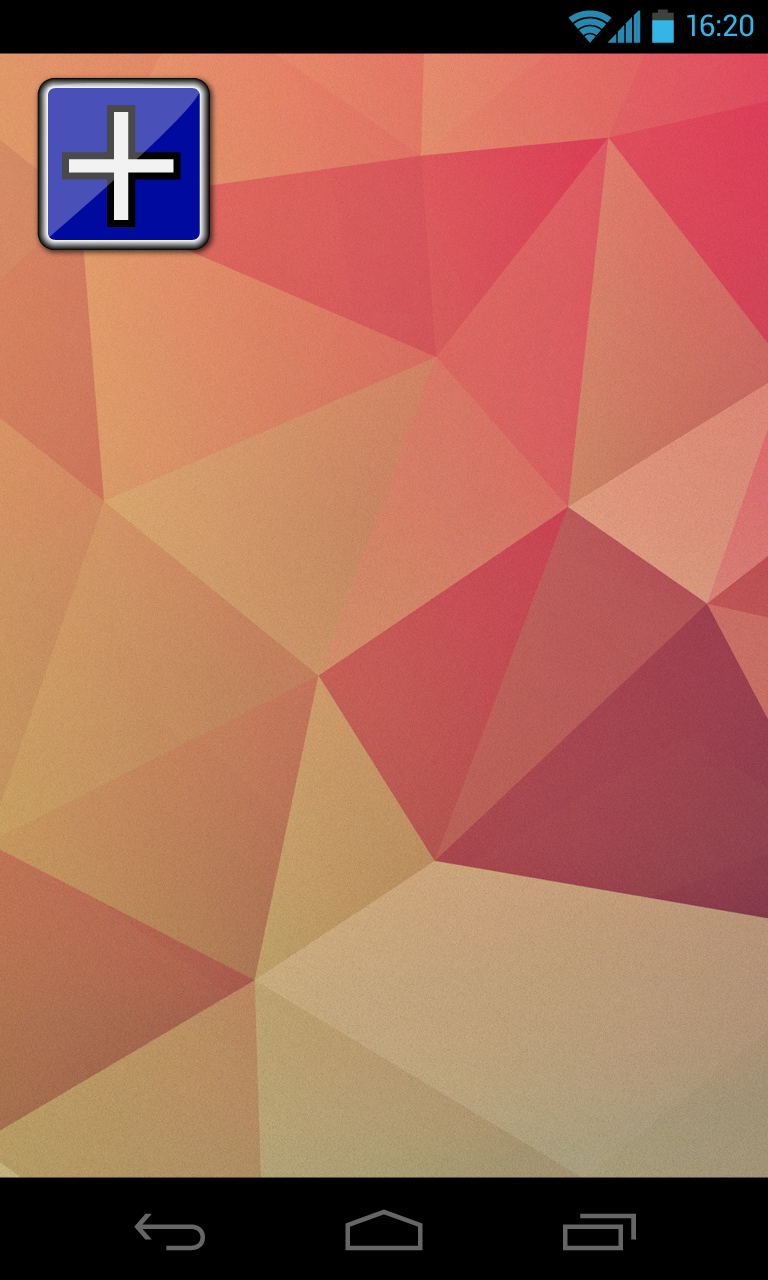
\includegraphics[scale=0.18]{Screens/00-Launch.png}

\includegraphics[scale=0.18]{Screens/00-Lock.png}
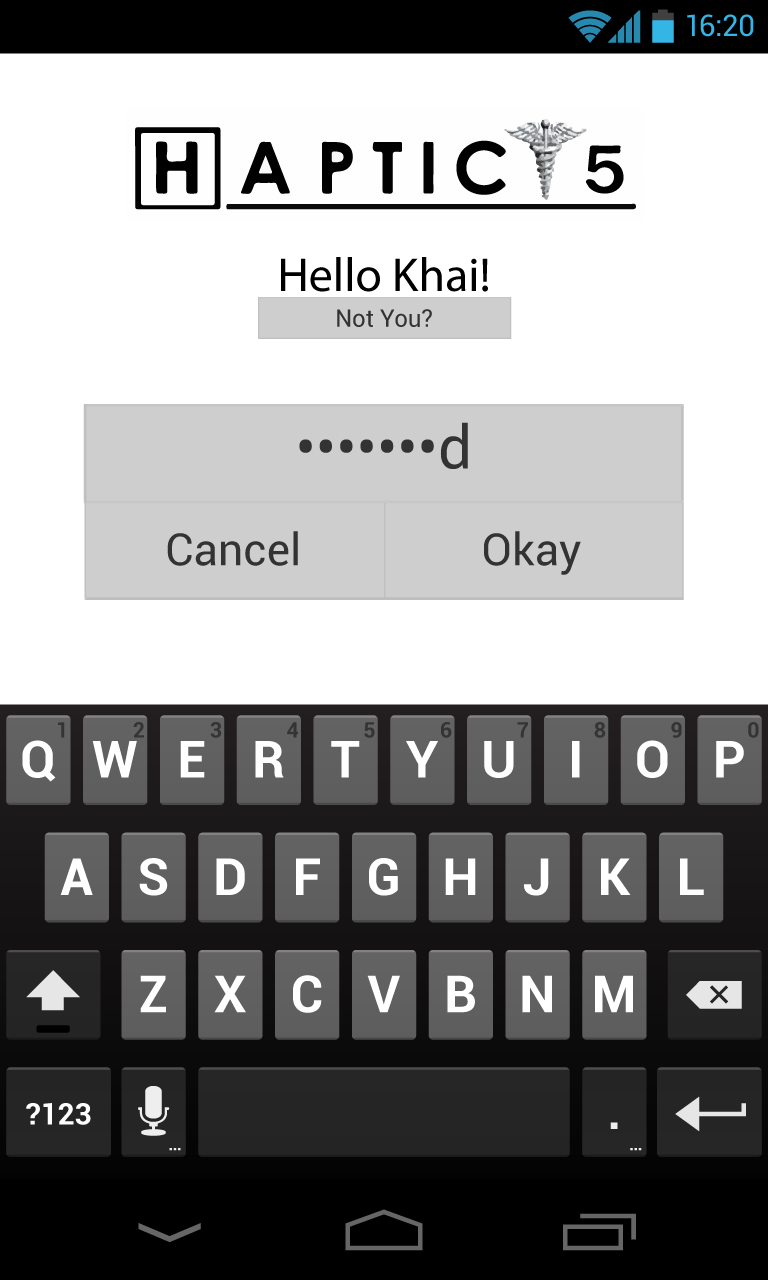
\includegraphics[scale=0.18]{Screens/00-Lock--Password-Entry.png}
\\\\
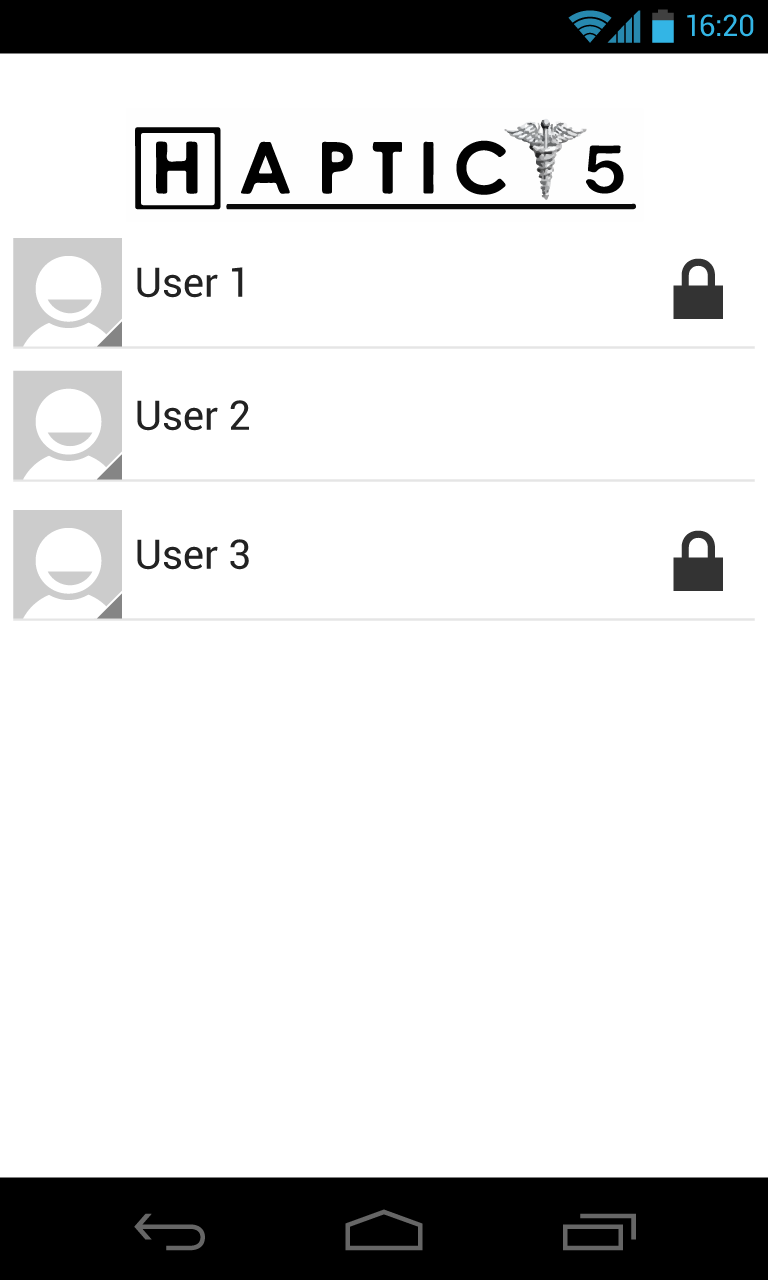
\includegraphics[scale=0.18]{Screens/01-Home---Change-User.png}
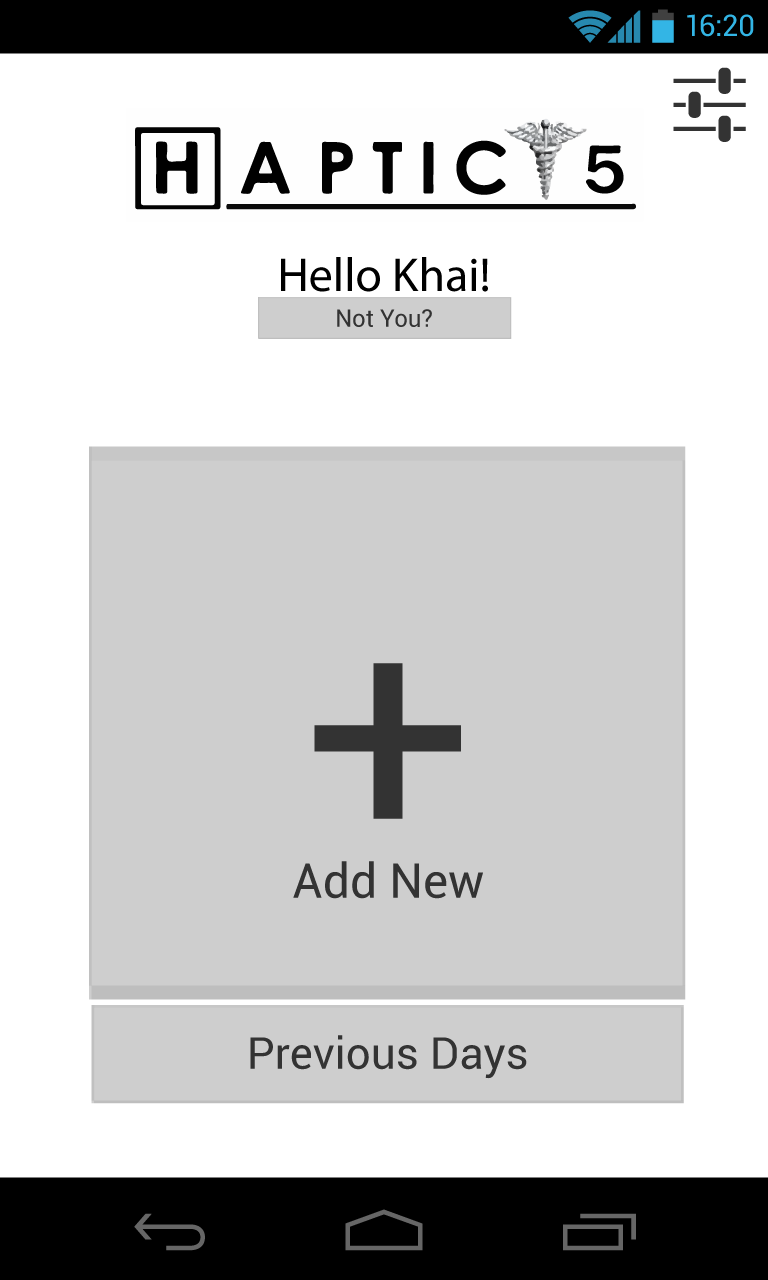
\includegraphics[scale=0.18]{Screens/01-Home---No-Selection.png}
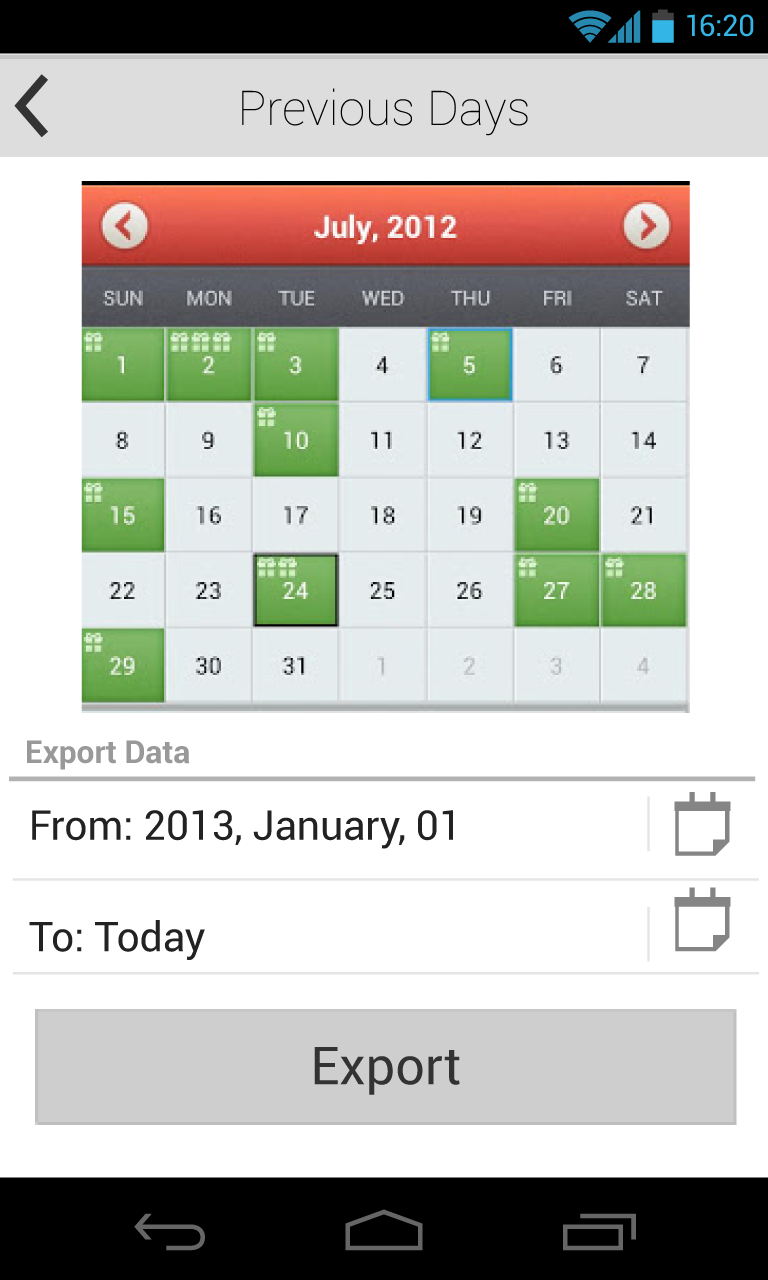
\includegraphics[scale=0.18]{Screens/02-Previous--No-Selection.png}
\\\\
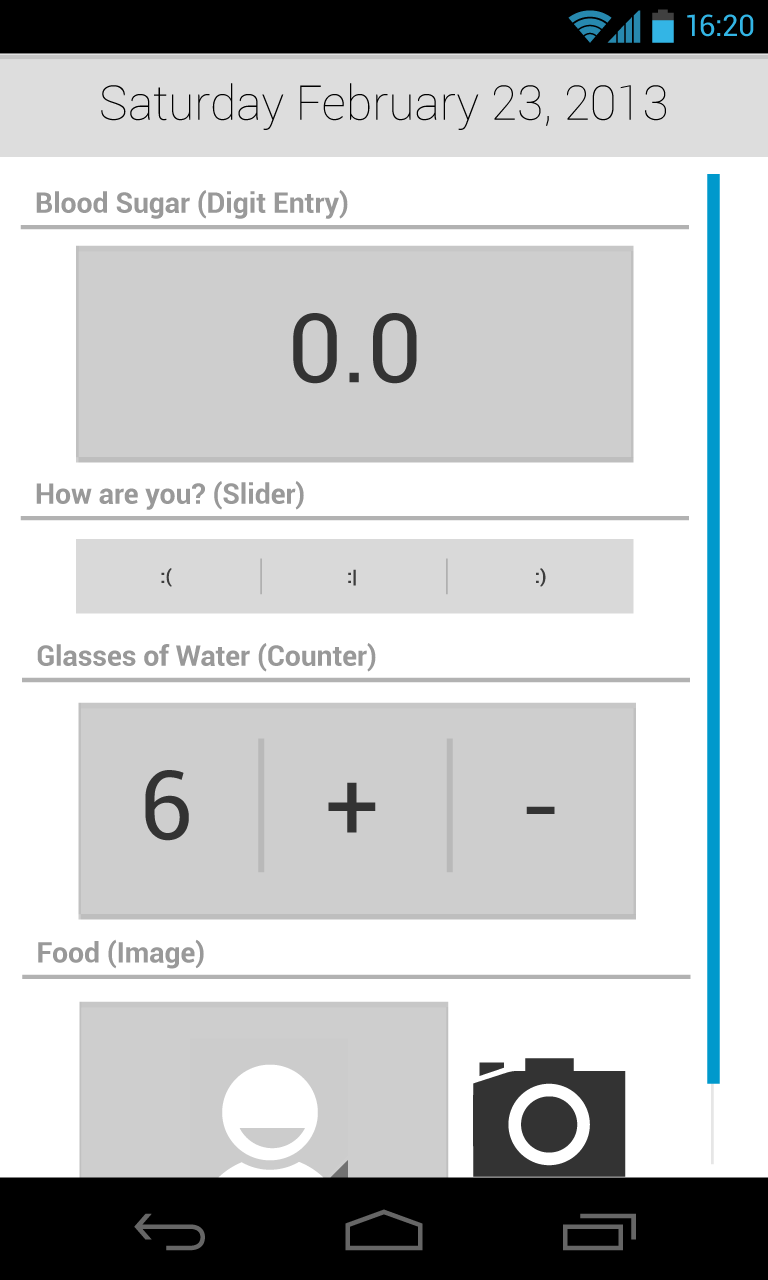
\includegraphics[scale=0.18]{Screens/03-Add--No-Selection.png}
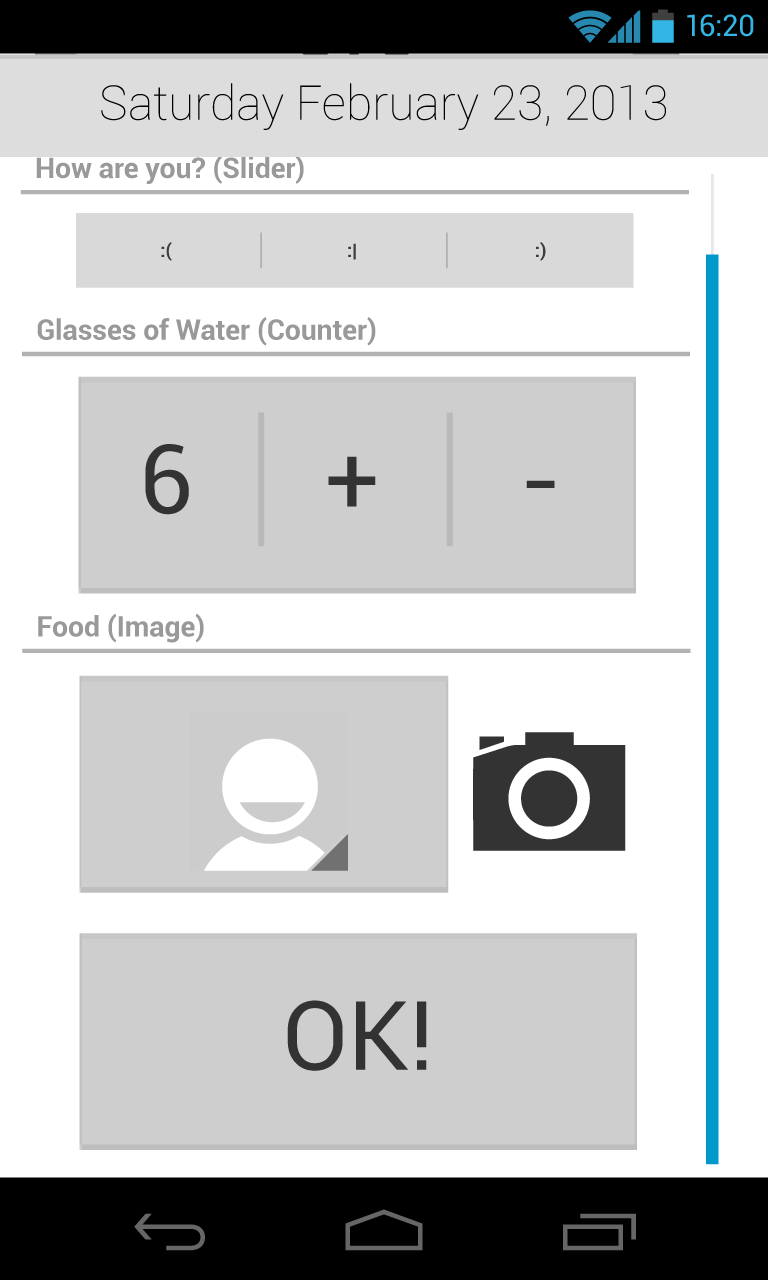
\includegraphics[scale=0.18]{Screens/03-Add--Scrolled.png}
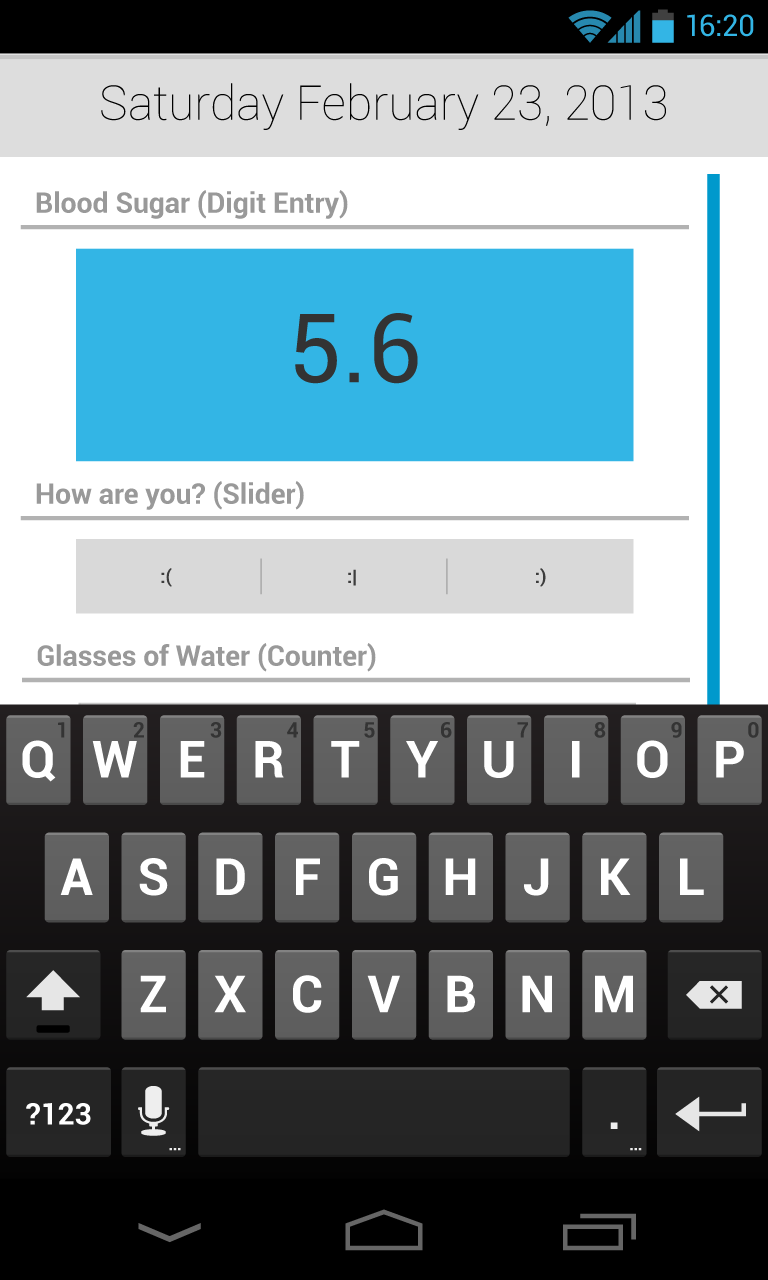
\includegraphics[scale=0.18]{Screens/03-Add--Add-Entry.png}
\\\\
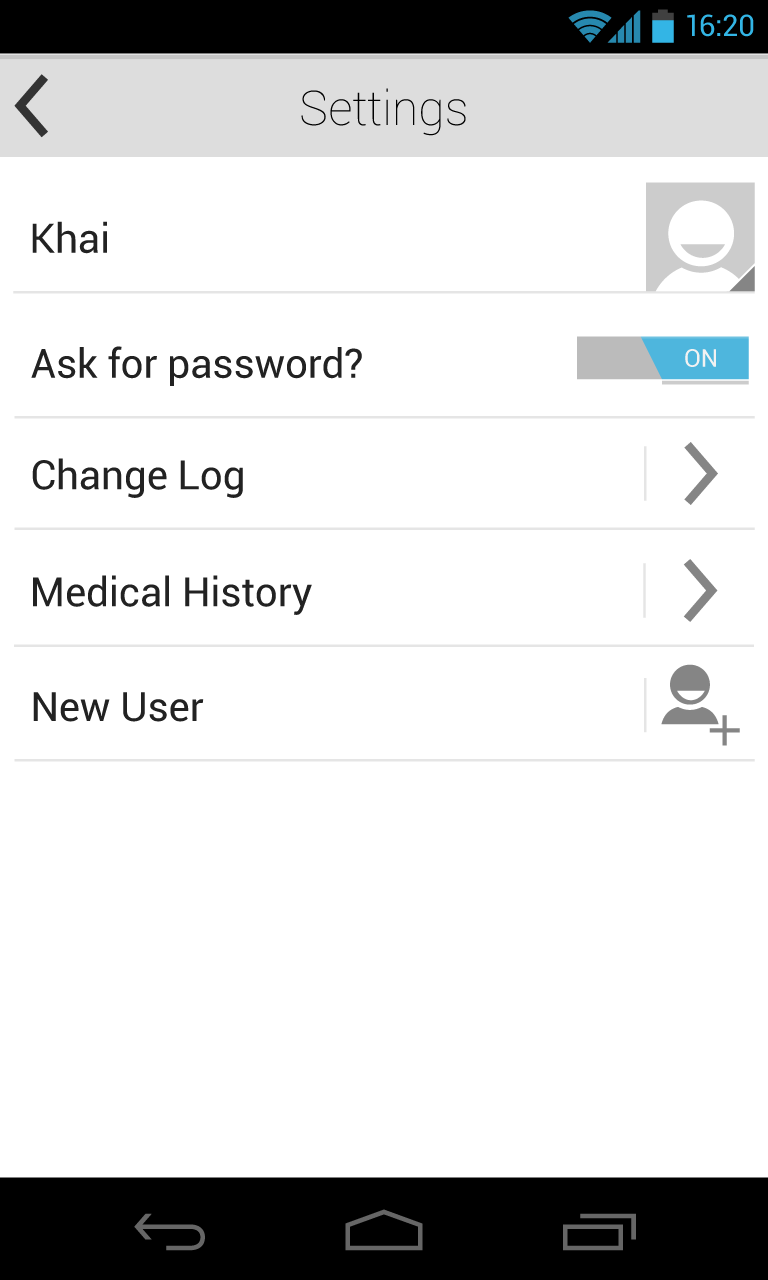
\includegraphics[scale=0.18]{Screens/04-Settings--Null.png}
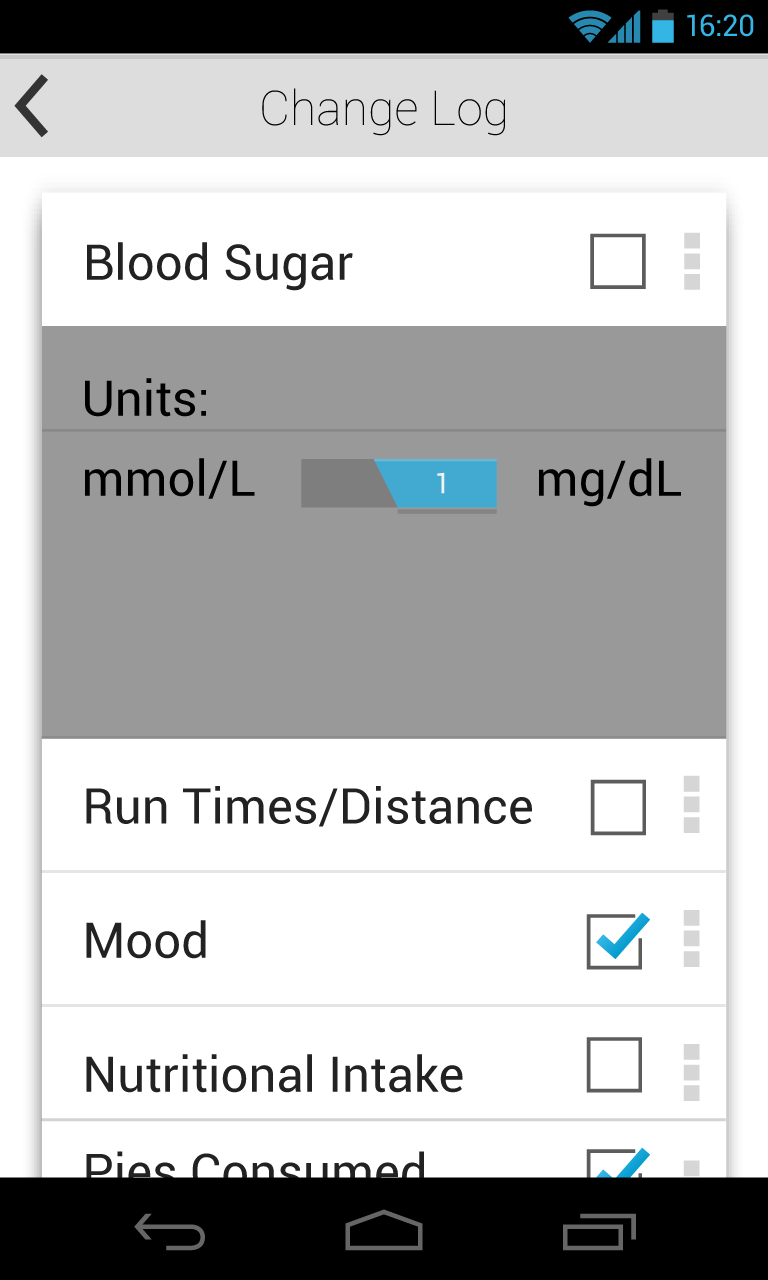
\includegraphics[scale=0.18]{Screens/05-Change-Log--Indi-Settings.png}
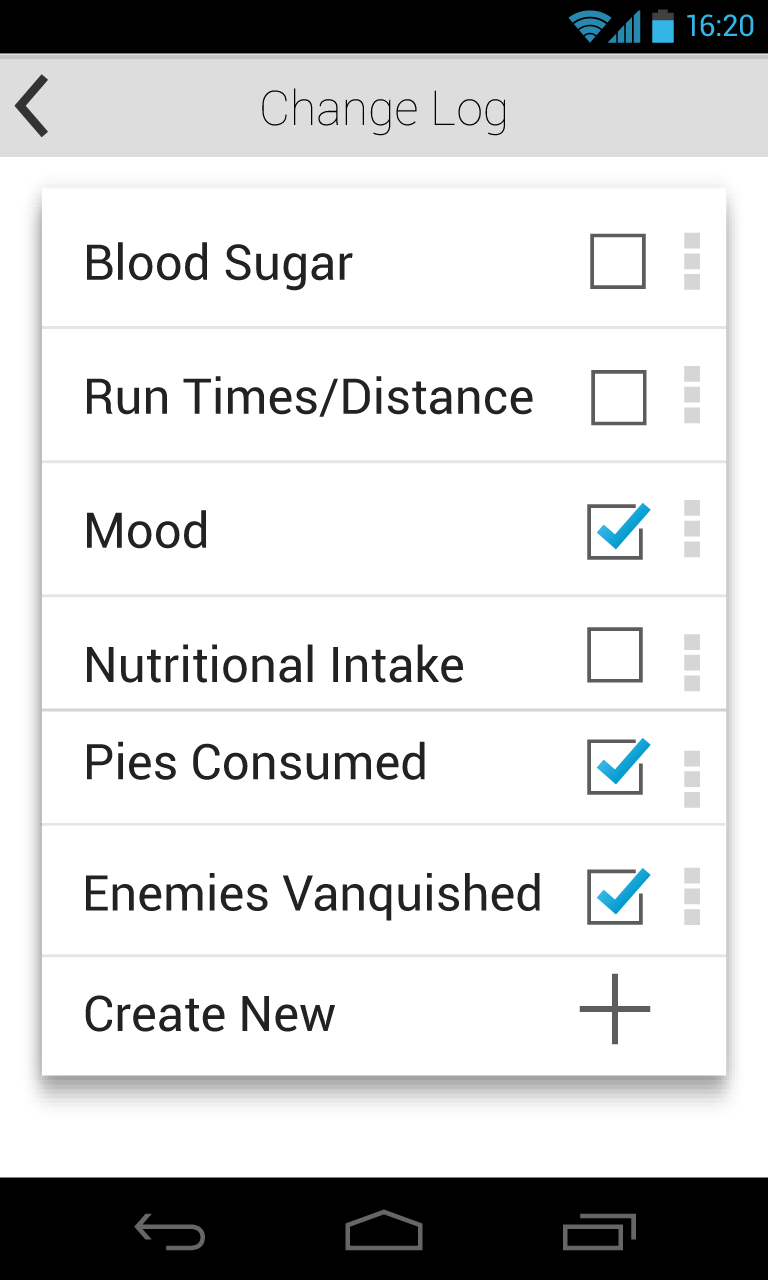
\includegraphics[scale=0.18]{Screens/05-Change-Log--Null.png}
\begin{enumerate}
\item{Phone Home Screen}
\item{Default User Screen (Password Protected)}
\item{Password Entry Screen}
\item{User Select Screen}
\item{User Home Screen}
\item{Previous Day Selection}
\item{Main Log Entry Screen}
\item{Main Log Entry Screen Scrolled Down}
\item{Selected Item Data Input}
\item{Settings Menu}
\item{Individual Category Customization}
\item{Category Menu}
\end{enumerate}



\end{document}
